% 本文件是示例论文的一部分
% 论文的主文件位于上级目录的 `main.tex`

\chapter{雨水资源GIS专题图详细设计与实现}

\section{功能设计}


\subsection{模块设计}
通过需求分析总体设计分析之后,将GIS专题图项目分为四个模块,主要为:大屏左面数据栏,右边数据栏,GIS专题图,头部导航栏四个模块,通过将数据展示栏和专题图还有导航栏分模块,可以使后期进行系统迭代更加方便,也符合模块化开发的标准和要求,主要模块分类如\ref{fig:module}所示:

\begin{figure}[!htb]%关于这些编译器的配置和使用,请参阅相关说明资料。
	\centering
	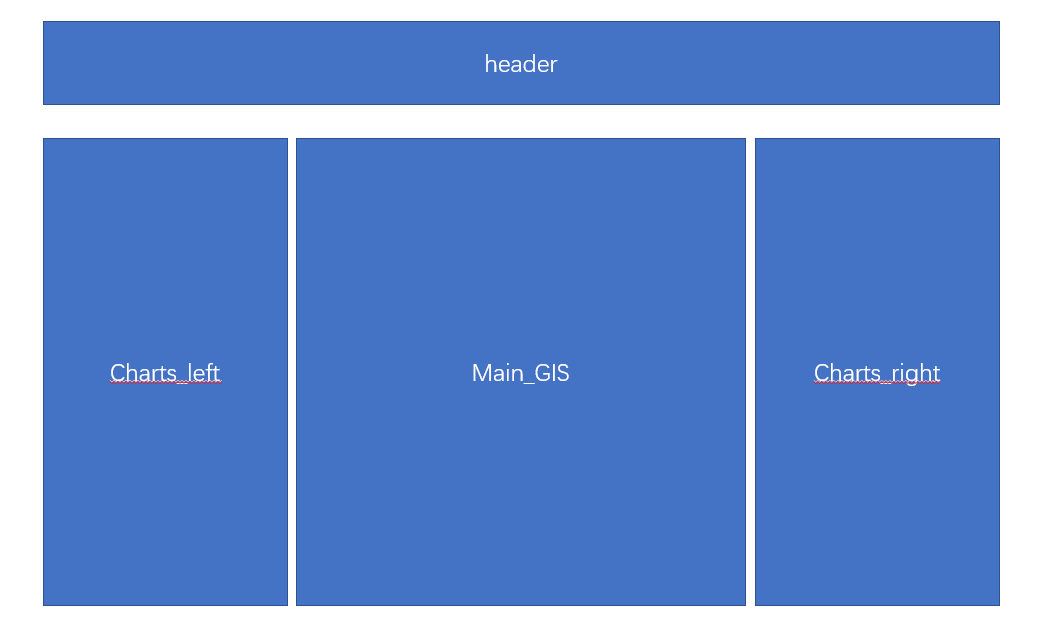
\includegraphics[width=0.60\textwidth]{figs/main.png}
	\caption{模块布局分类}
	\label{fig:module}
\end{figure}

\subsection{界面设计}
界面设计如\ref{fig:jiemian}所示:

\begin{figure}[!htb]%关于这些编译器的配置和使用,请参阅相关说明资料。
	\centering
	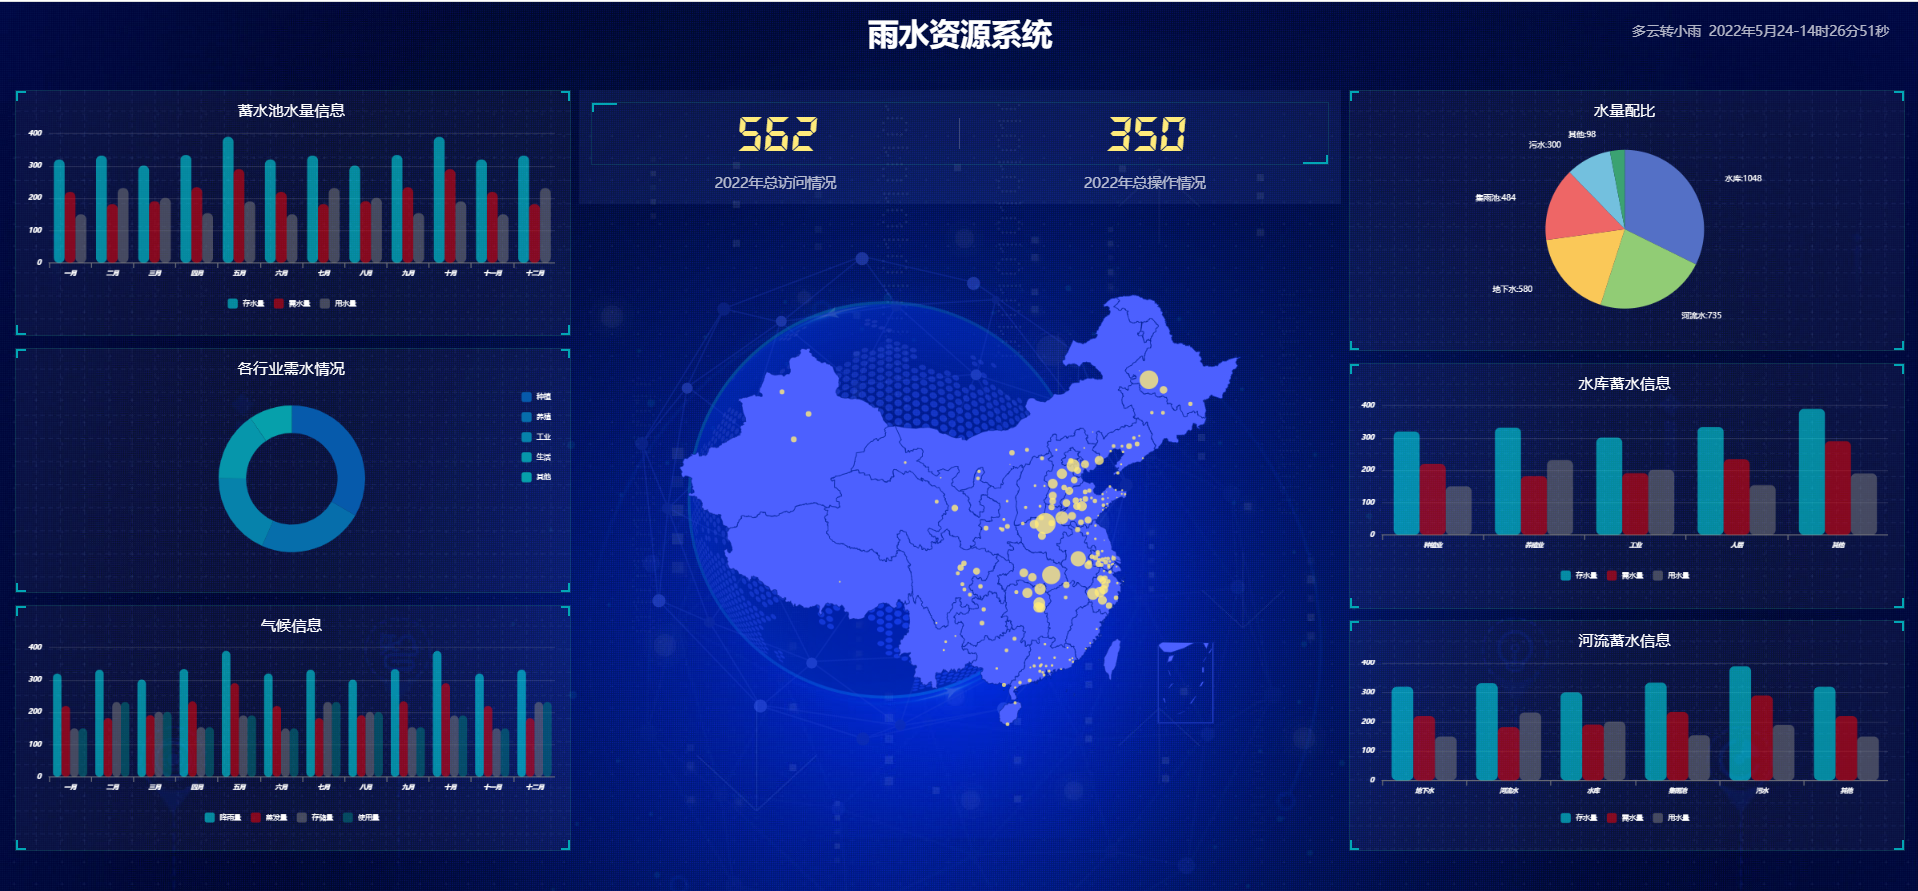
\includegraphics[width=0.60\textwidth]{figs/jiemian.png}
	\caption{界面设计}
	\label{fig:jiemian}
\end{figure}
\subsection{QGIS底图设计}
首先通过QGIS从世界地图中截取本题目需要的中国地图,此世界地图使用的是网上开源地图数据,如\ref{fig:ditu}所示。

\begin{figure}[!htb]%关于这些编译器的配置和使用,请参阅相关说明资料。
	\centering
	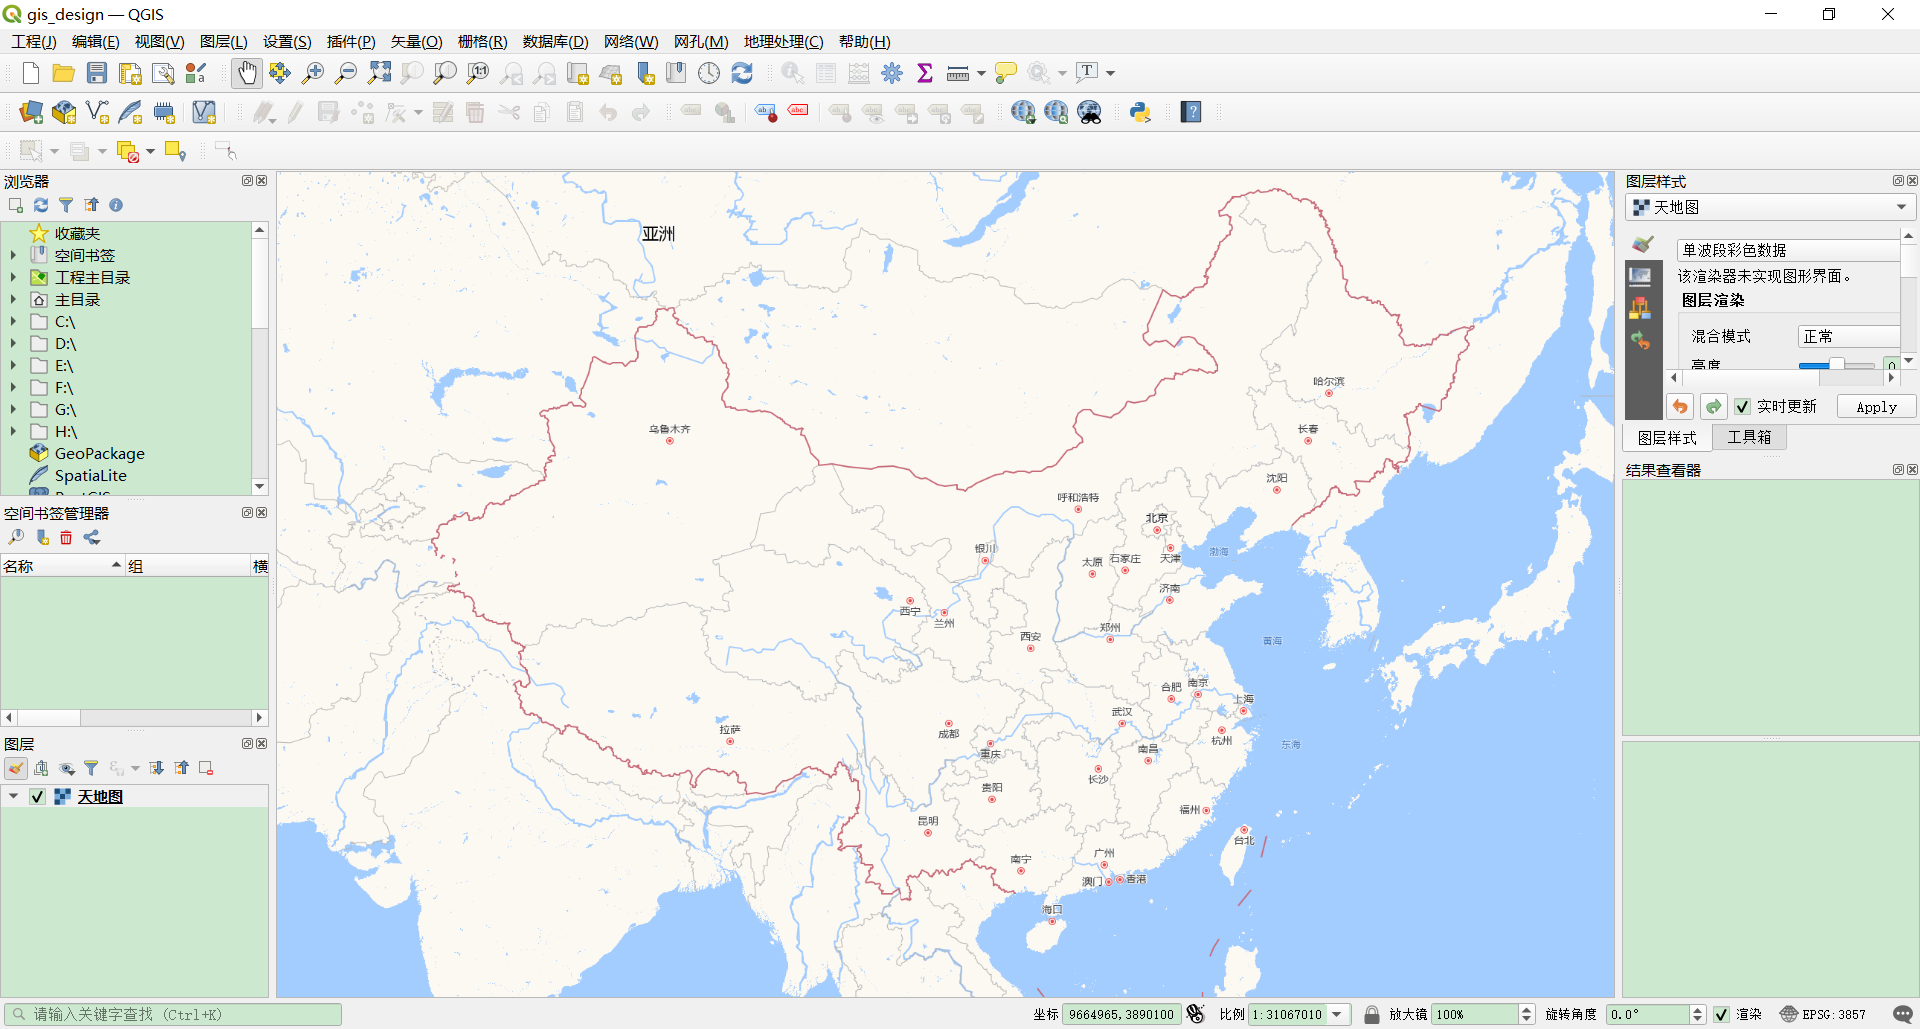
\includegraphics[width=0.60\textwidth]{figs/gisditu.png}
	\caption{底图加载}
	\label{fig:ditu}
\end{figure}
通过QGIS自带的截取功能将世界地图截取需求所需要的各种地图,截取的其中之一如\ref{fig:shezhiditu}所示。
\begin{figure}[!htb]%关于这些编译器的配置和使用,请参阅相关说明资料。
	\centering
	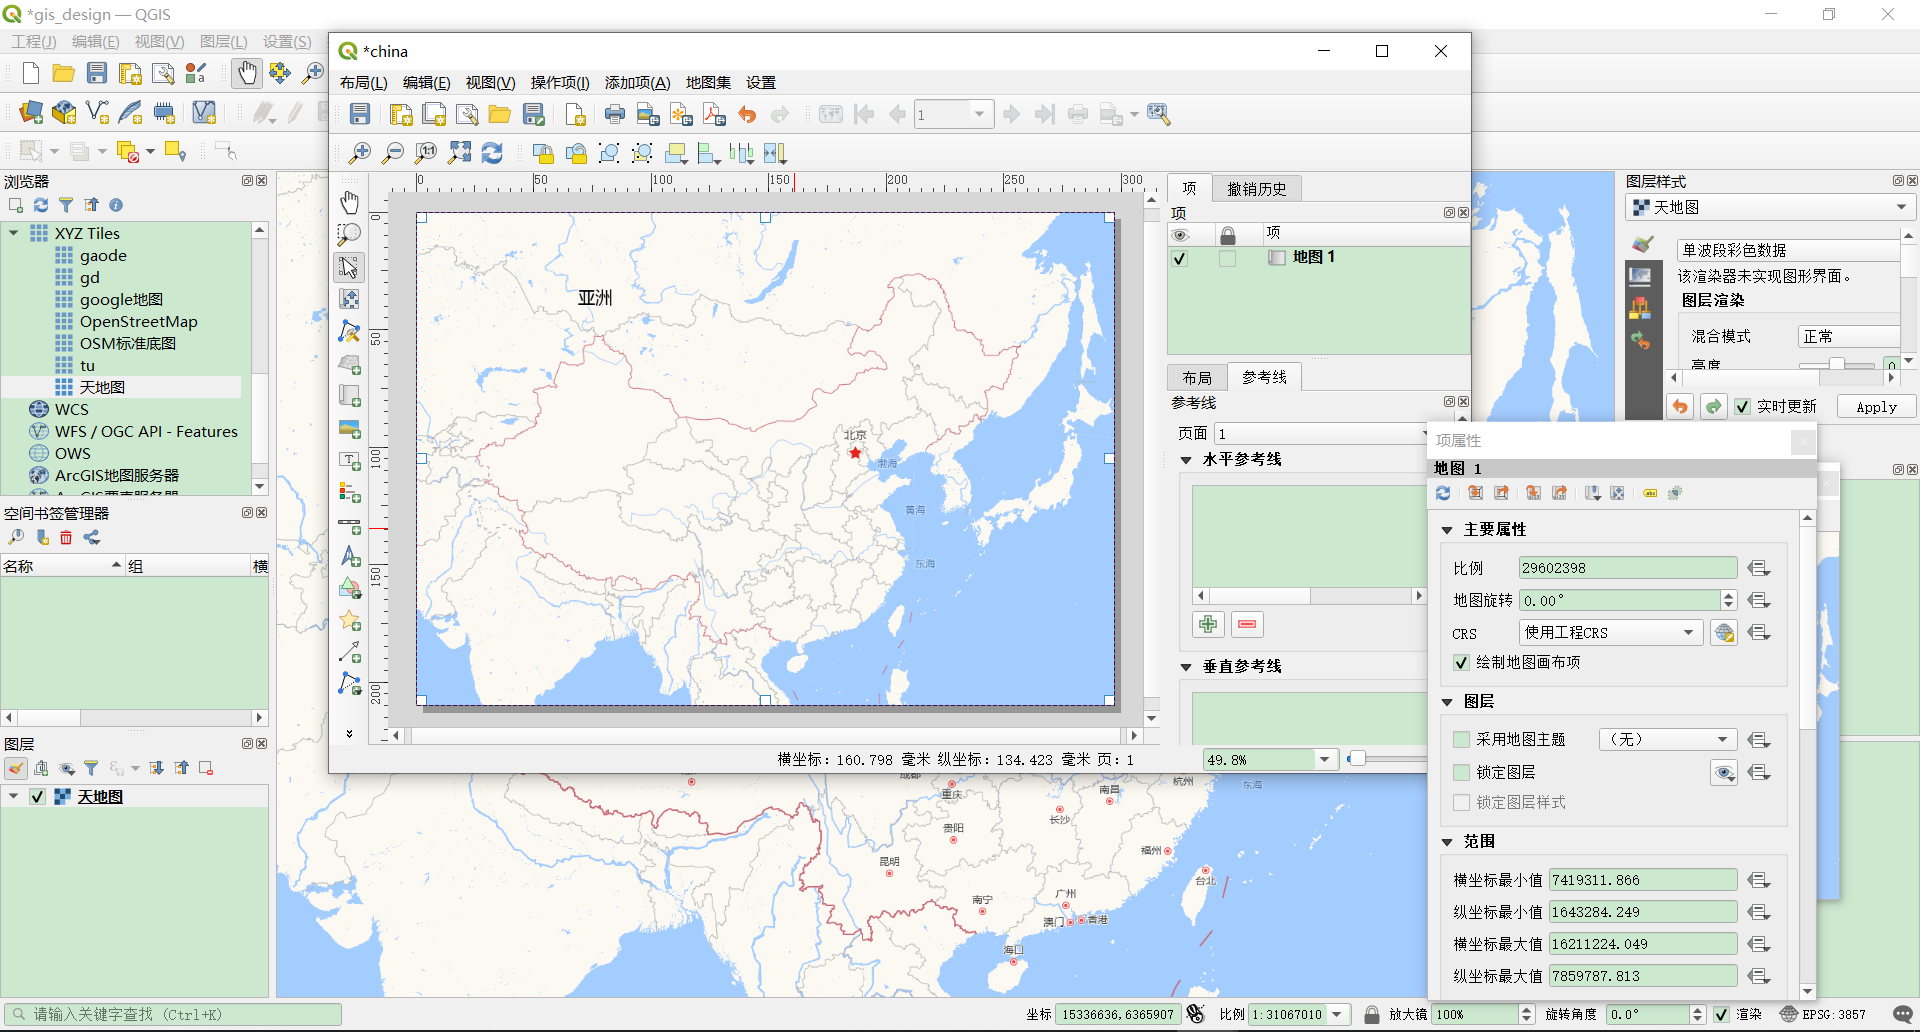
\includegraphics[width=0.60\textwidth]{figs/shezhiditu.png}
	\caption{地图截取}
	\label{fig:shezhiditu}
\end{figure}
\subsection{部署GeoServer}
使用geoserver进行地图发布,我们主要选择了shp数据文件作为GeoServer的数据文件进行发布,首先创建工作区,这样使之后创建的所有的地图图层数据全部发布至本工作区内,方便之后使用OpenLayers调用各种地图,创建工作区如\ref{fig:gongzuoqu}所示。
\begin{figure}[!htb]%关于这些编译器的配置和使用,请参阅相关说明资料。
	\centering
	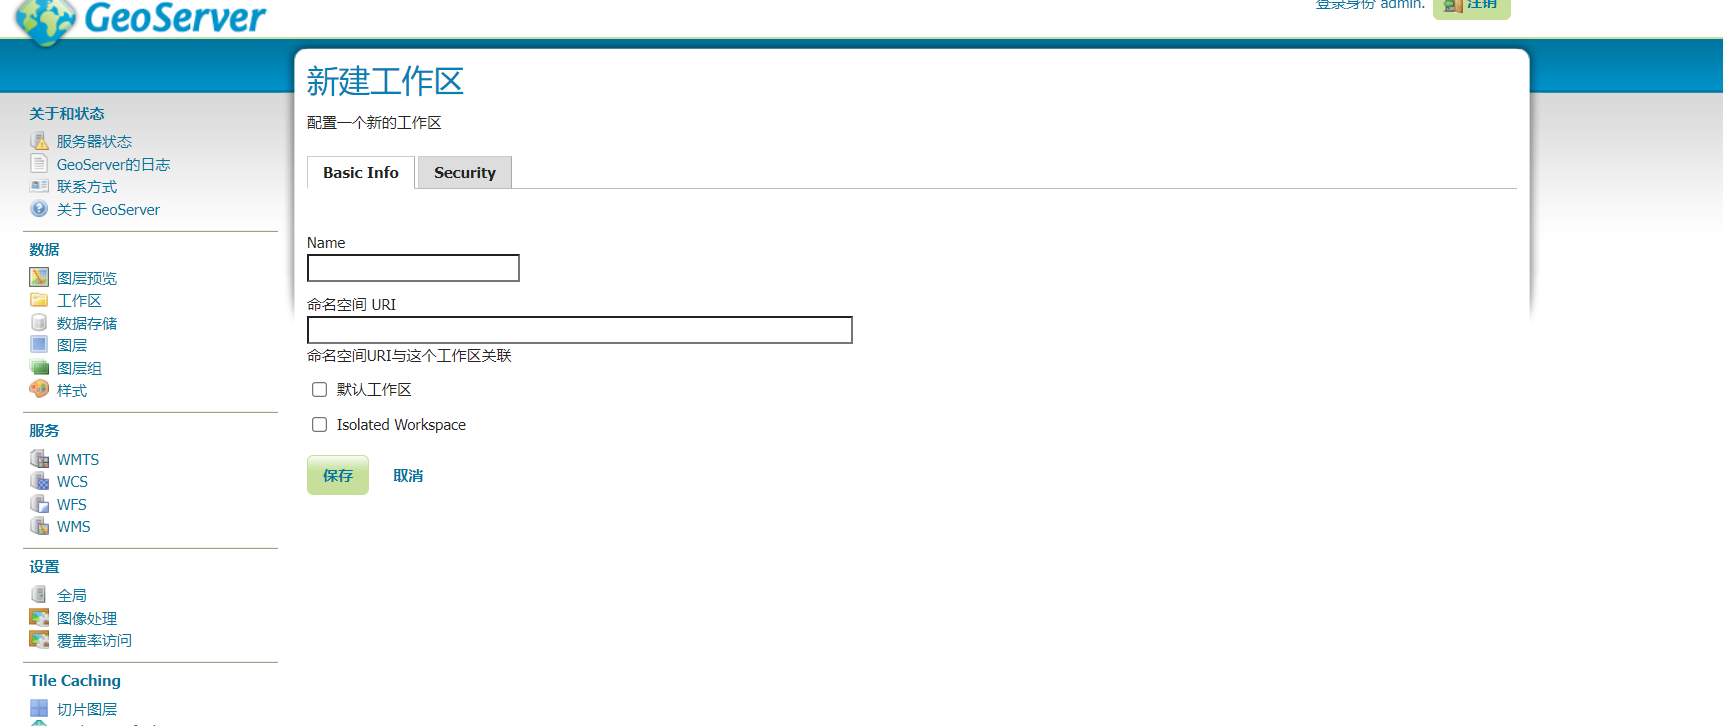
\includegraphics[width=0.60\textwidth]{figs/创建工作区.png}
	\caption{创建工作区}
	\label{fig:gongzuoqu}
\end{figure}
创建完工作区之后,就可以进行数据文件的上传,首先通过QGIS导出文件之后,将文件长传到GeoServer上,选择数据源如\ref{fig:xinjianshuju}所示。
\begin{figure}[!htb]%关于这些编译器的配置和使用,请参阅相关说明资料。
	\centering
	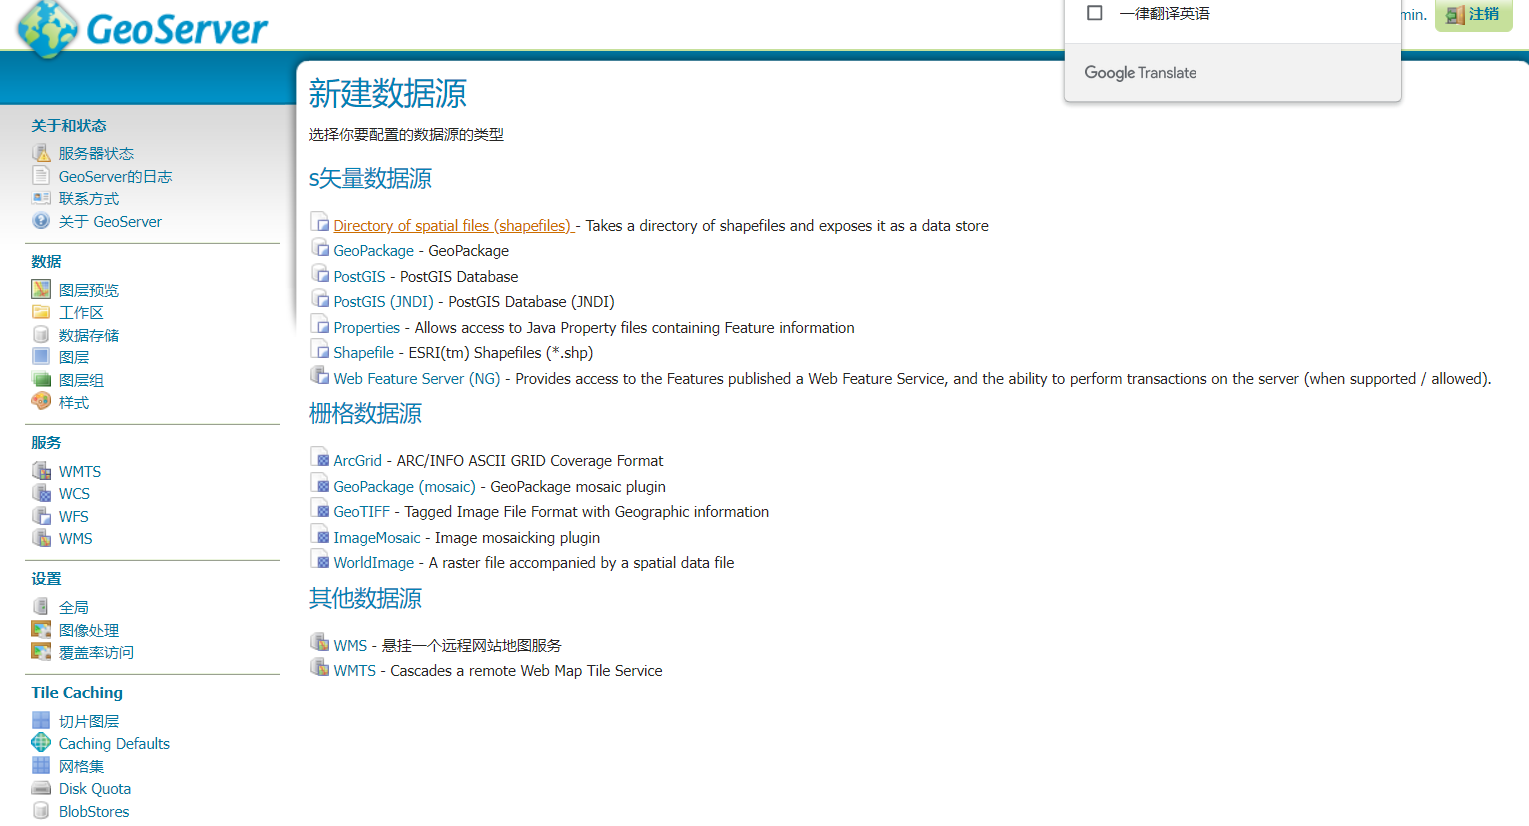
\includegraphics[width=0.60\textwidth]{figs/新建数据.png}
	\caption{导入数据}
	\label{fig:xinjianshuju}
\end{figure}

导入数据文件如\ref{fig:tianjiawenjian}所示:

\begin{figure}[!htb]%关于这些编译器的配置和使用,请参阅相关说明资料。
	\centering
	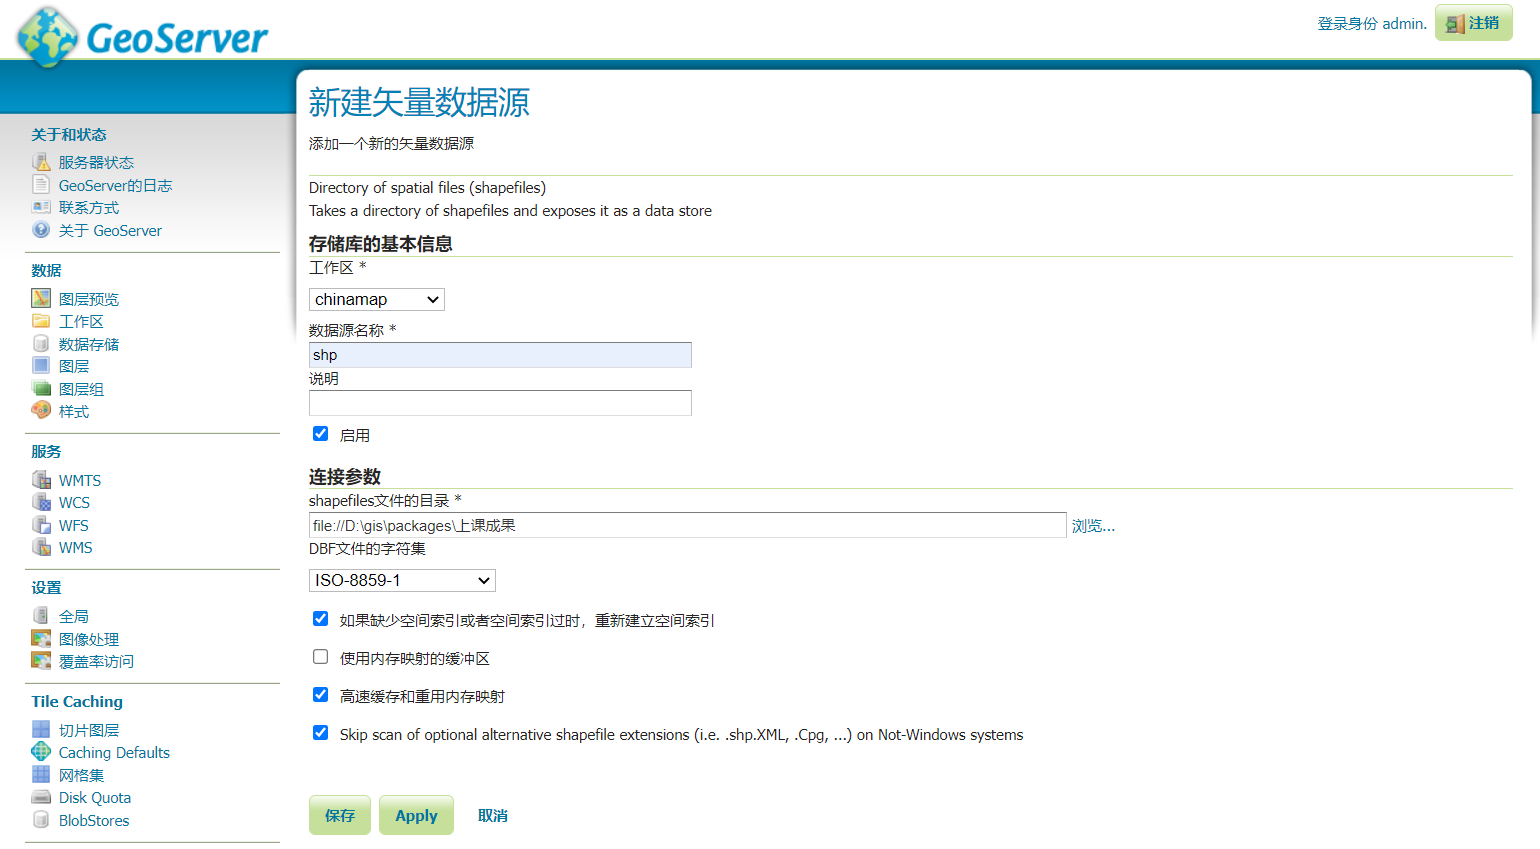
\includegraphics[width=0.60\textwidth]{figs/添加文件.png}
	\caption{导入文件}
	\label{fig:tianjiawenjian}
\end{figure}
导入数据文件之后,我们还需要进行坐标系的选取,这样才能真正的将地图文件导入至geoserver里。操作如\ref{fig:zuobiaoxi}所示。
\begin{figure}[!htb]%关于这些编译器的配置和使用,请参阅相关说明资料。
	\centering
	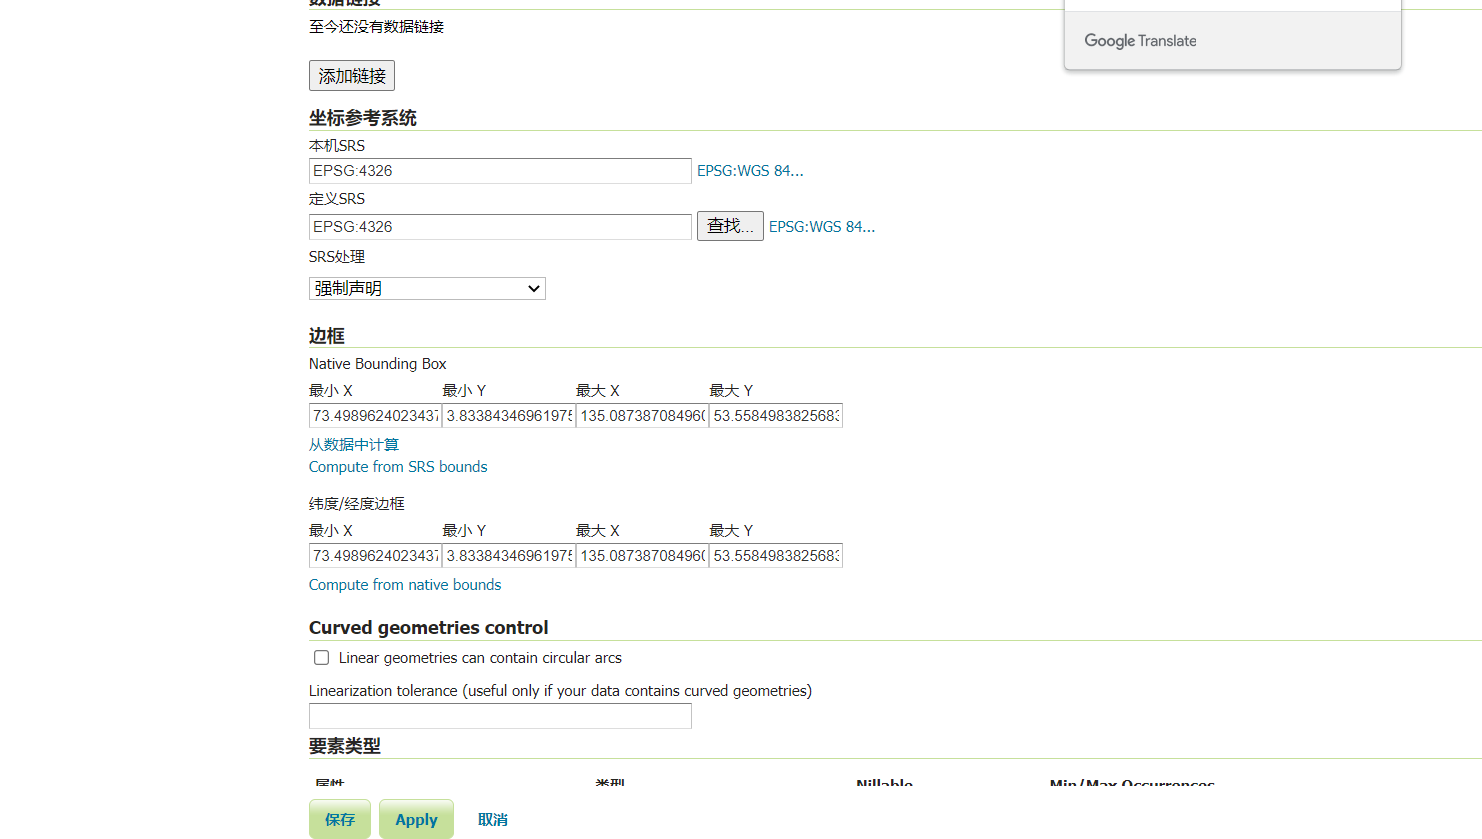
\includegraphics[width=0.60\textwidth,height=0.2\textheight]{figs/zuobiaoxi.png}
	\caption{选取坐标系}
	\label{fig:zuobiaoxi}
\end{figure}
\subsection{OpenLayers渲染}
1.第一步,首先通过OpenLayers调取发布在GeoServer上的地图图层,主要设置参数有:service,version,request ,typeName,output\_options。然后使用ajax获取json数据,因为GeoServer的输出格式就是json文件。

2.第二步,通过OpenLayers的getZoomForResolution,getLonLatFromViewPortPx,getViewPortPxFromLonLat,moveTo,zoomToMaxExtent,zoomToScale等方法给地图添加方法缩小比例尺转化,设置分辨率等基本功能。

3.第三步,对地图进行点线面渲染,主要通过ol.style.Circle,ol.style.Icon,ol.style.Stroke,ol.style.Fill,ol.style.Stroke等操作,对地图进行需求所需的渲染。

\section{地表水系设计}

\subsection{河流专题图设计}
河流专题图主要是体现出河流的流量信息,以便观测河流是否会产生旱涝灾害,以及能利用的河流水信息,由于传感器的设计是检测河流中的某个点的流量,因此对于整条河流的流量会有差异,为了更好地显示,设计了河流不同分段展示不同流量信息,并且通过河流的颜色深浅变化来直观的观测河流的流量大小,基本展示如\ref{fig:heliu}所示。当数据产生变化时,该专题图可以随着数据动态变化这里展示当长江下游流量产生变化时,专题图的变化效果,这里将流量变化量增大一些,这样可以更直观的观察到专题图的动态变化效果,如\ref{fig:heliubianhua}所示。
\begin{figure}[!htb]%关于这些编译器的配置和使用,请参阅相关说明资料。
	\centering
	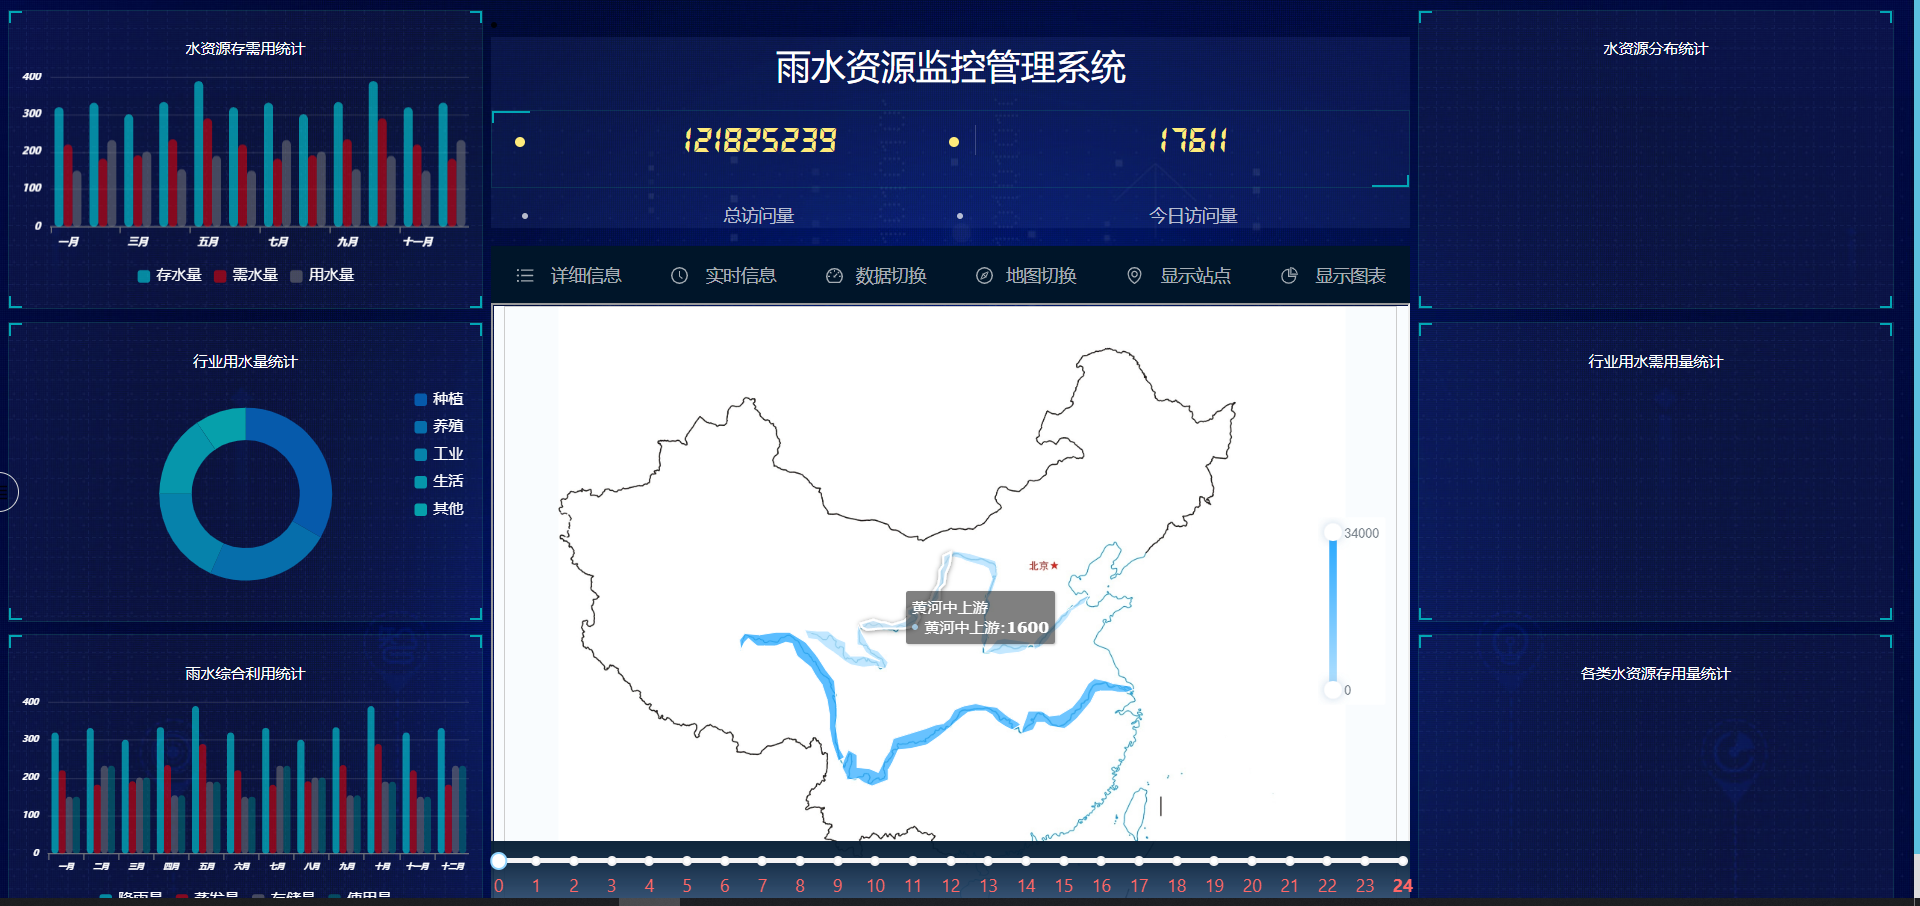
\includegraphics[width=0.60\textwidth]{figs/river_1.png}
	\caption{河流专题图}
	\label{fig:heliu}
\end{figure}

\begin{figure}[!htb]%关于这些编译器的配置和使用,请参阅相关说明资料。
	\centering
	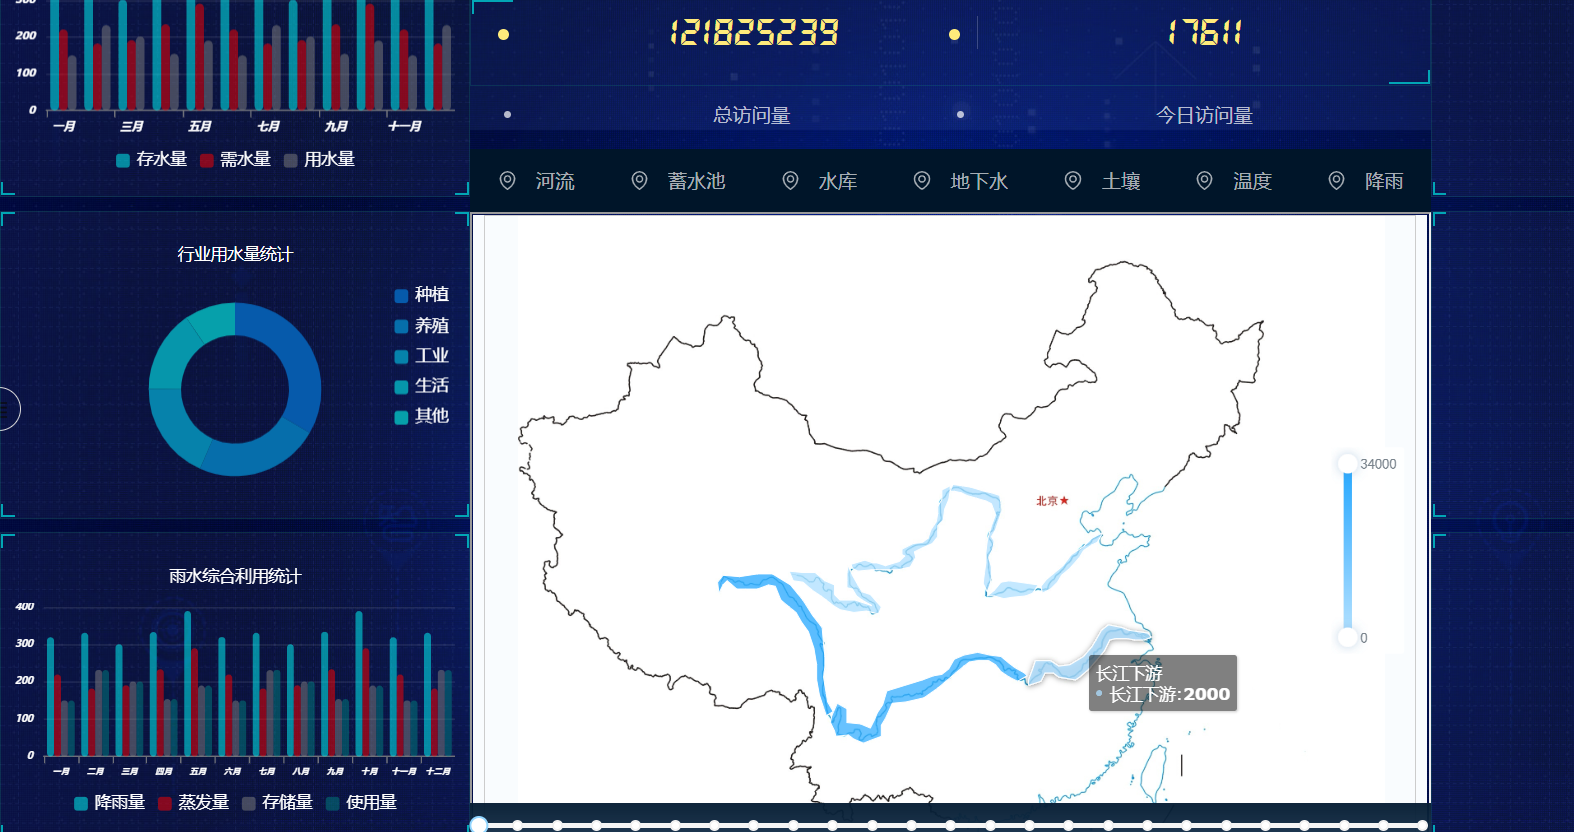
\includegraphics[width=0.60\textwidth]{figs/bianhua.png}
	\caption{河流流量变化专题图}
	\label{fig:heliubianhua}
\end{figure}
\subsection{蓄水池专题图设计}
蓄水池专题图主要体现出蓄水池的储水量的信息,以便很容易的观测出蓄水池的储水量信息,使得相关人员根据蓄水池储水量信息合理的调配水资源,实现合理高效利用水资源的目的,对于蓄水池的储水量来说,点状信息已经足够,所以通过点密度专题图可以做出符合要求的蓄水池专题图,本专题图还采用了3D地图显示,可以使得相关人员更好的观测信息,并且可以实现数据的动态更新,当数据库中的数据更新时,专题图的数据信息也会产生相应变化,例如添加了新的蓄水池信息,在地图上就会动态的添加新的蓄水池标记,还有如果蓄水池的数据变化,专题图也会相应的变化数据信息,基本展示如\ref{fig:xushuici}所示。
\begin{figure}[!htb]%关于这些编译器的配置和使用,请参阅相关说明资料。
	\centering
	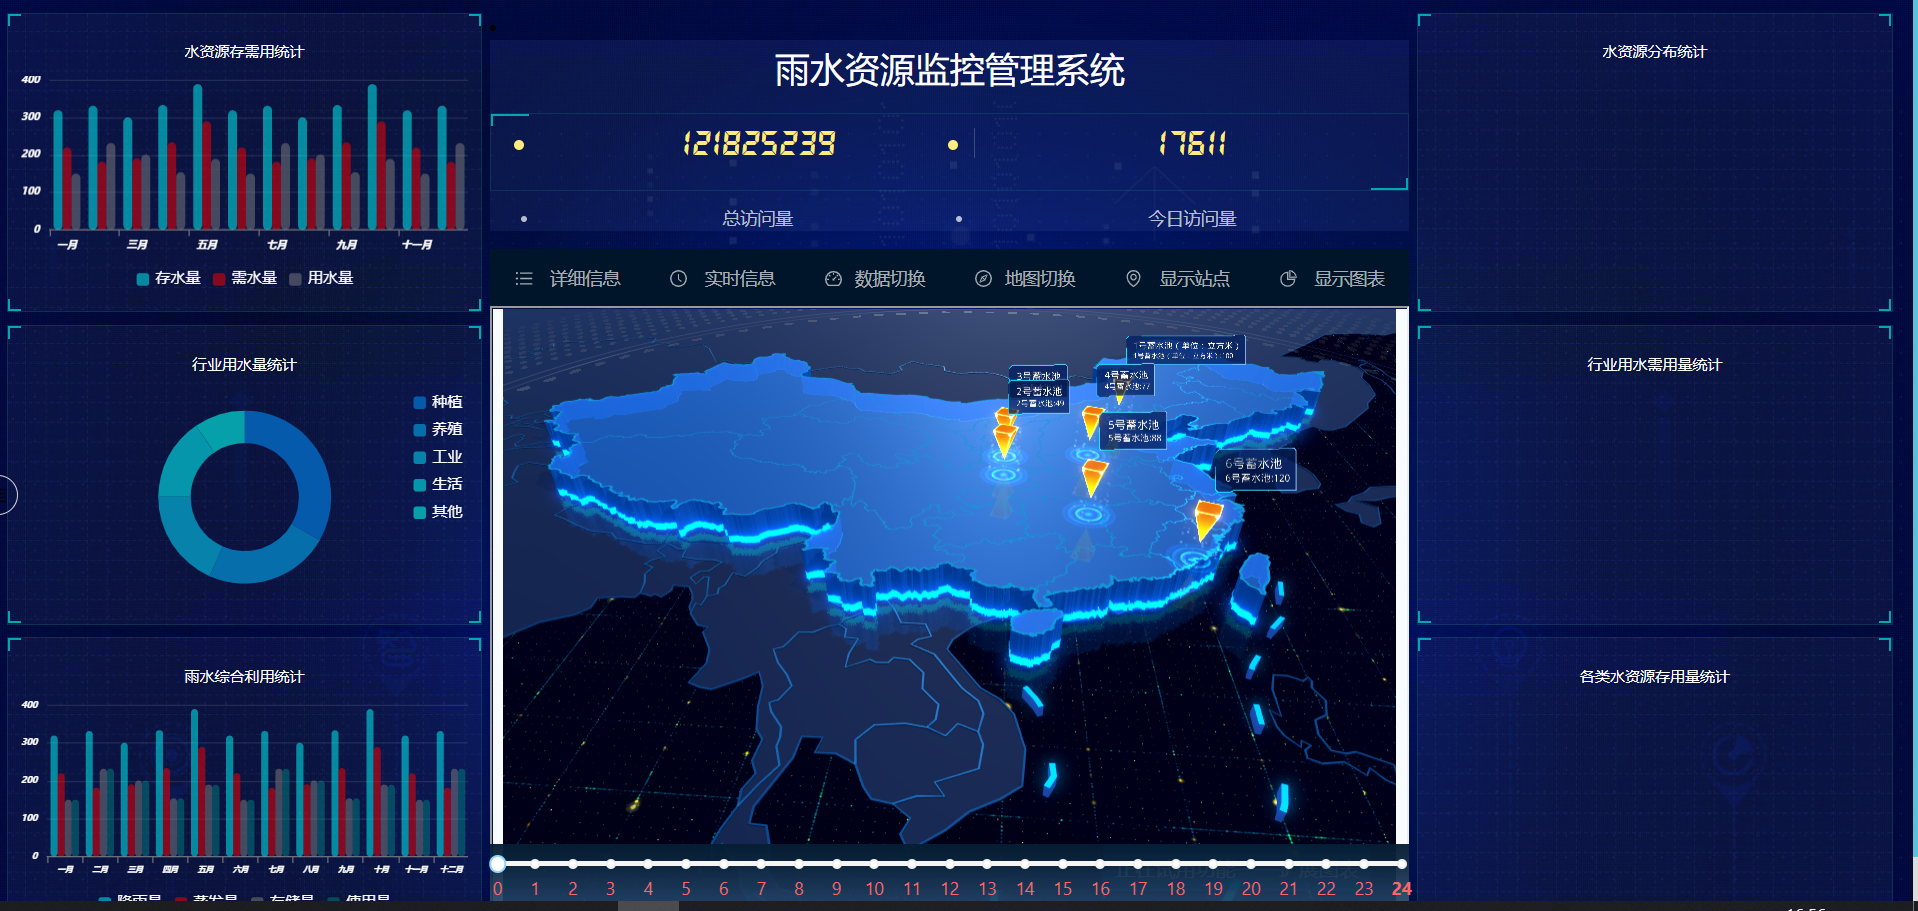
\includegraphics[width=0.60\textwidth]{figs/xushuici.png}
	\caption{蓄水池专题图}
	\label{fig:xushuici}
\end{figure}
\subsection{水库专题图设计}
水库的专题图与蓄水池专题图类似,也是主要展示水库的储水量的信息,需求与目的也和蓄水池类似,直观的反映出水库的储水量信息,以便相关人员进行水资源的调配以及合理高效利用。与蓄水池专题图一样,也是使用了3D地图,数据也可以动态更新,当时水库信息添加,水库数据变化时,专题图都会产生相应的变化,基本展示如\ref{fig:shuiku}所示。
\begin{figure}[!htb]%关于这些编译器的配置和使用,请参阅相关说明资料。
	\centering
	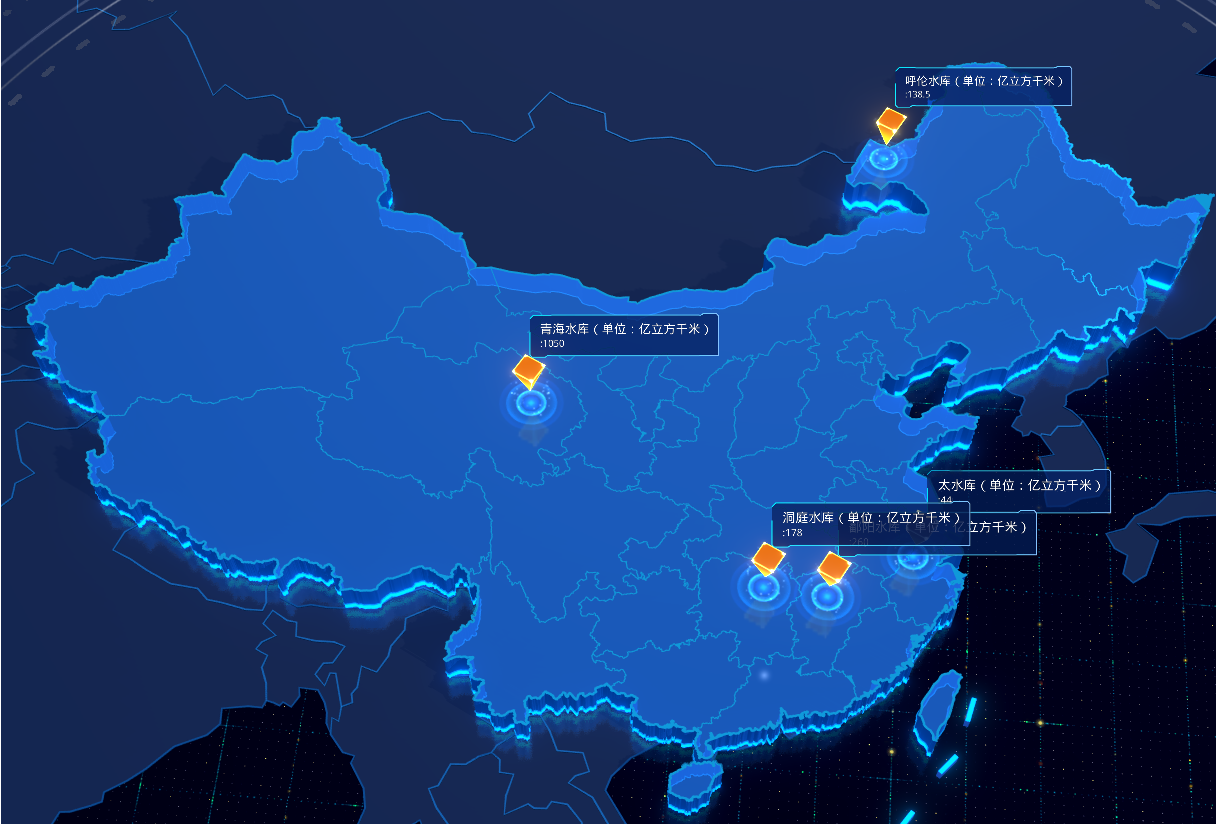
\includegraphics[width=0.60\textwidth]{figs/shuiku.png}
	\caption{水库专题图}
	\label{fig:shuiku}
\end{figure}
\section{地下水系设计}
\subsection{地下水分布专题图}
地下水分布构造十分复杂,使用GIS专题图很难直观的展示出地下水的分布信息,因此地下水分布专题图采用了行政区归属这一信息进行专题图的制作,主要是通过测出每个行政区域地下水含量信息,通过每个行政区这一区域粒度来展示地下水的信息,地下水的信息也会根据传感器测得的数据的变化而变化,基本展示如\ref{fig:dixiashui}所示。
\begin{figure}[!htb]%关于这些编译器的配置和使用,请参阅相关说明资料。
	\centering
	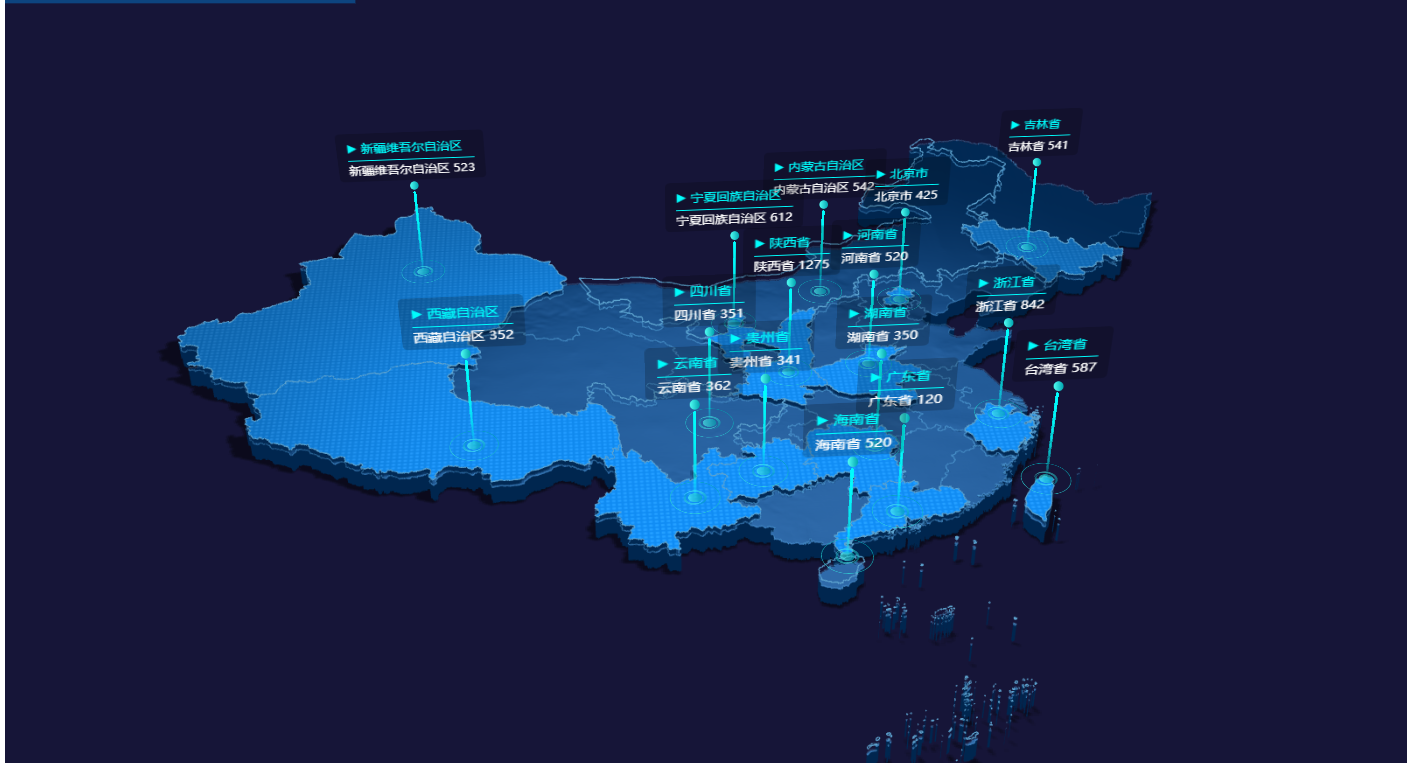
\includegraphics[width=0.60\textwidth]{figs/dixiashui.png}
	\caption{地下水专题图}
	\label{fig:dixiashui}
\end{figure}
\subsection{土壤类型和土壤含量专题图}
土壤类型和土壤含量专题图主要通过区域粒度来展示土壤类型与含量信息,土壤类型通过不同颜色来表示,一种颜色代表着一种土壤类型,当鼠标或者在大屏上用手触摸到某一个区域时,便会展示土壤具体含量信息,土壤具体含量信息也会根据数据的变化而产生的相应的变化,相关人员通过查看相关土壤信息可以合理的安排作物的种植等,基本展示如\ref{fig:turang}所示,\ref{fig:turang}所示为从中国地图展示各省份的土壤信息,当区域粒度更小时,使用地图钻取的效果可以使得土壤信息更加小区域化,这里以山东省为例,中国地图如\ref{fig:zuanqu}所示,当点击山东区域时,便会钻入山东省地图,展示各市的土壤信息,如\ref{fig:shandong}所示。
\begin{figure}[!htb]%关于这些编译器的配置和使用,请参阅相关说明资料。
	\centering
	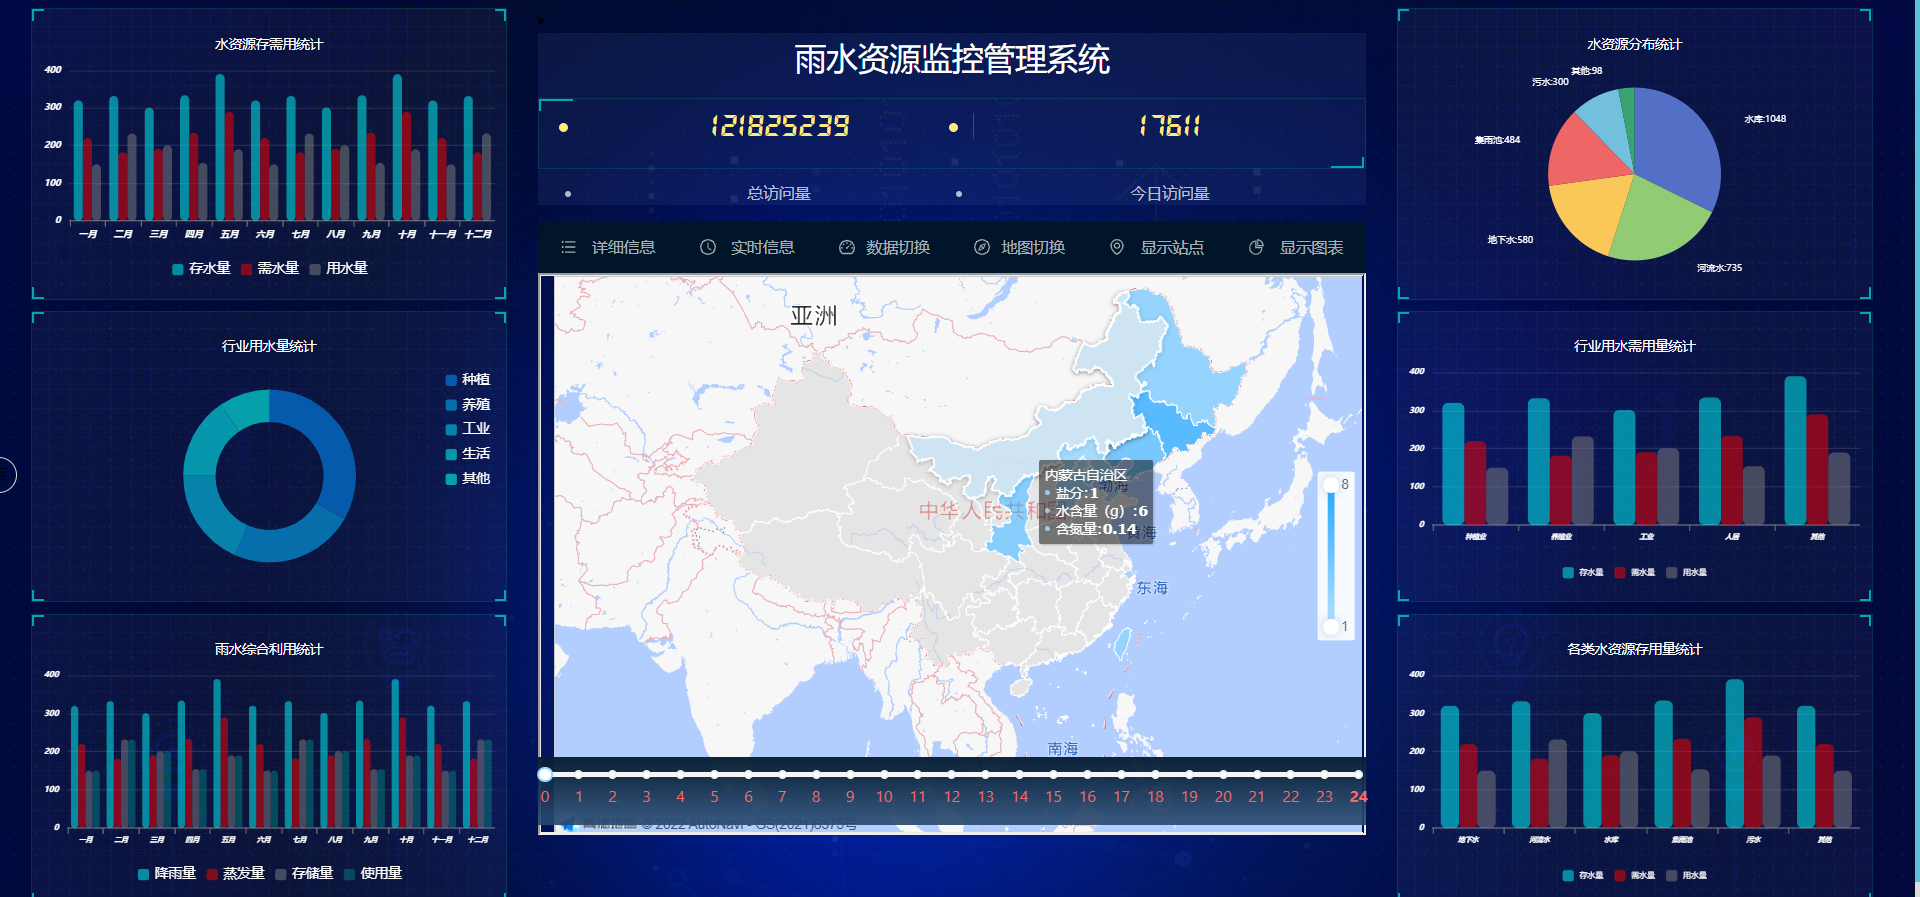
\includegraphics[width=0.60\textwidth]{figs/turang.png}
	\caption{土壤专题图}
	\label{fig:turang}
\end{figure}
\begin{figure}[!htb]%关于这些编译器的配置和使用,请参阅相关说明资料。
	\centering
	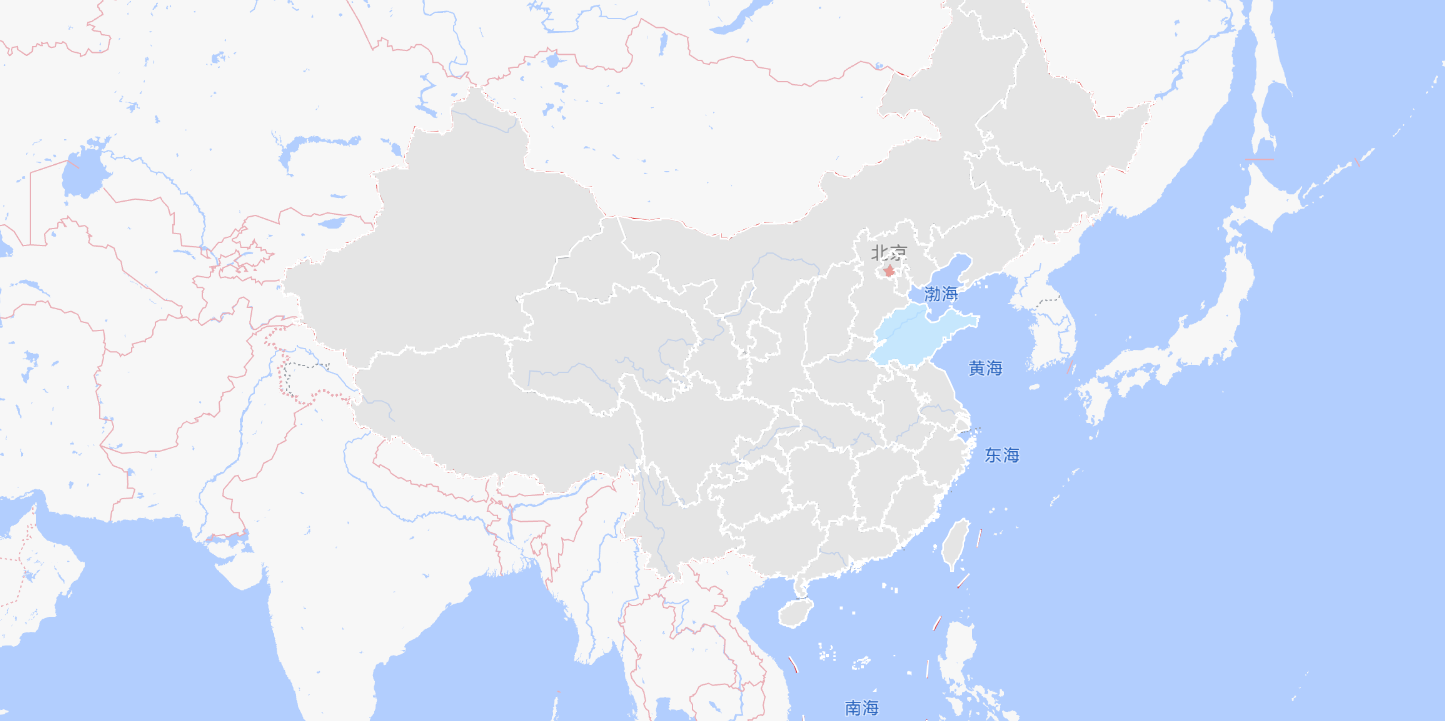
\includegraphics[width=0.60\textwidth]{figs/shili.png}
	\caption{地图钻取示例}
	\label{fig:zuanqu}
\end{figure}
\begin{figure}[!htb]%关于这些编译器的配置和使用,请参阅相关说明资料。
	\centering
	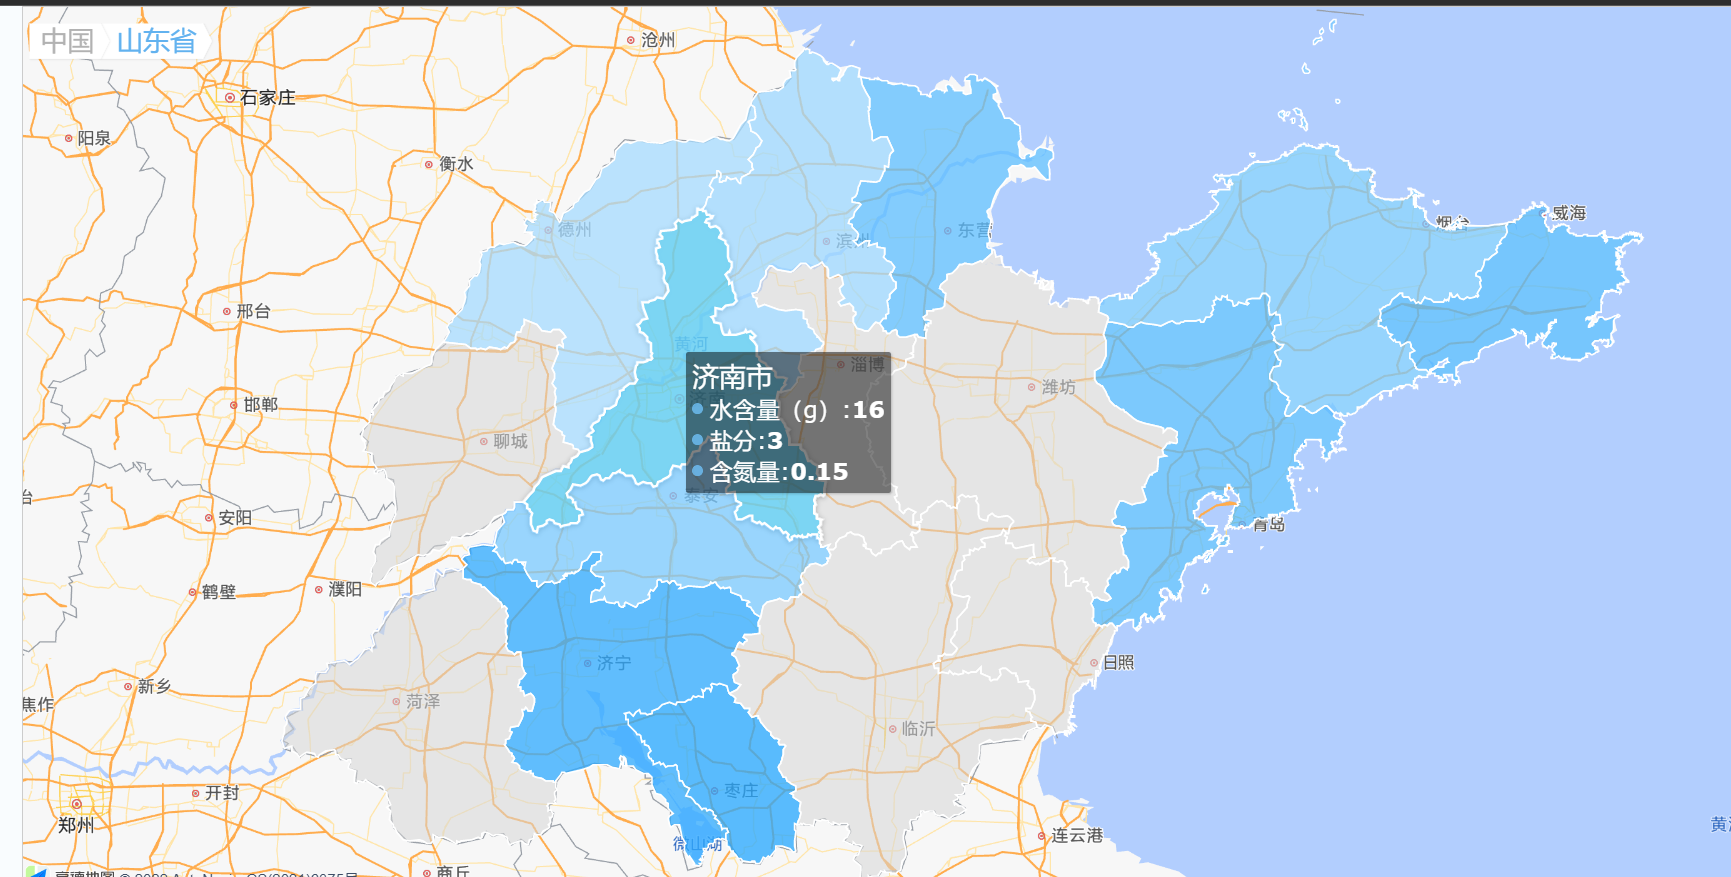
\includegraphics[width=0.60\textwidth]{figs/shandong.png}
	\caption{钻入后的山东地图}
	\label{fig:shandong}
\end{figure}

\section{气候图}
\subsection{温度专题图}
温度专题图主要展示地区的温度信息,因为温度信息是区域性质的,因此需要设计范围专题图来直观的展示温度高低的信息,并通过颜色的渐变来展示温度高低,因为温度随着时间会动态变化,因此该专题图也会根据数据的变化产生相应实时的变化,基本展示如\ref{fig:wendu}所示。
\begin{figure}[!htb]%关于这些编译器的配置和使用,请参阅相关说明资料。
	\centering
	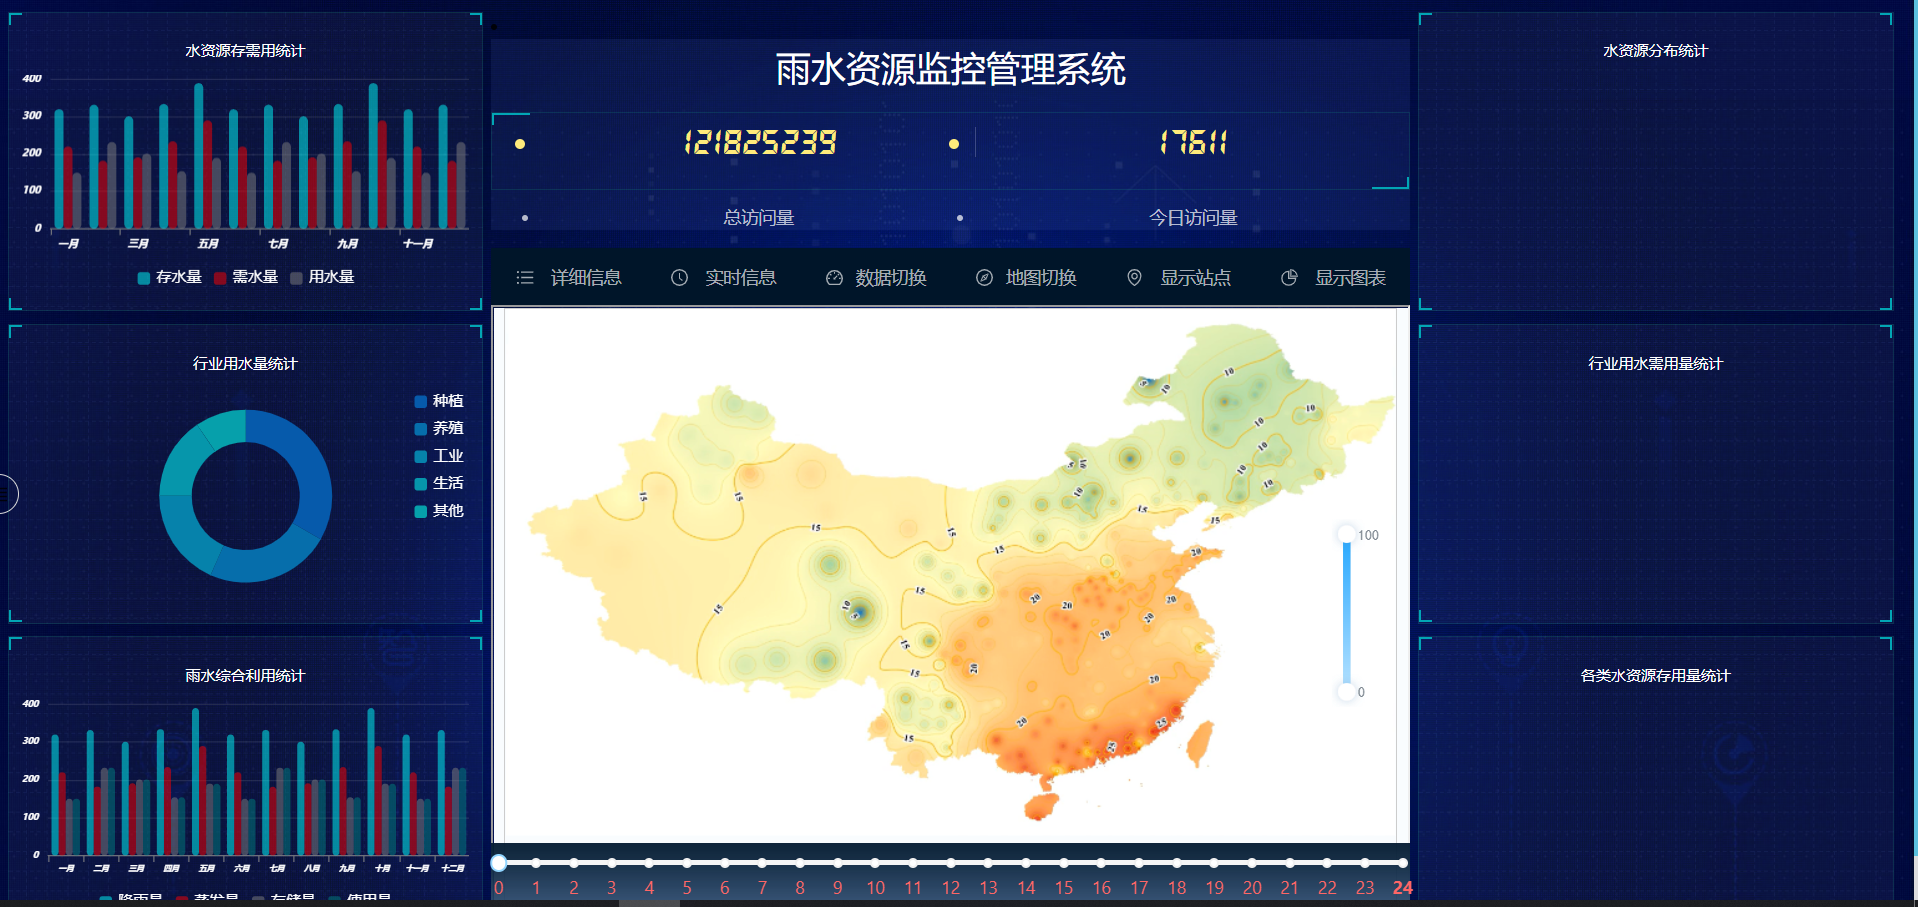
\includegraphics[width=0.60\textwidth]{figs/温度图.png}
	\caption{温度专题图}
	\label{fig:wendu}
\end{figure}
\subsection{降雨专题图}
降雨专题图也是区域性质的,因此与温度专题图一样需要设计范围专题图,主要通过颜色的深浅来表示降雨大小的信息,不过与温度专题图差异的地方在于降雨专题图的区域不是将整个中国区域都覆盖,因为降雨的特点,会通过降雨的区域信息来对地图进行区域覆盖,降雨区域会通过颜色的深浅表示降雨的大小,当鼠标点击降雨地区时,会展示实时的降雨量信息,并且根据数据的变化产生相应的变化,基本展示如\ref{fig:jiangyu}所示.
\begin{figure}[!htb]%关于这些编译器的配置和使用,请参阅相关说明资料。
	\centering
	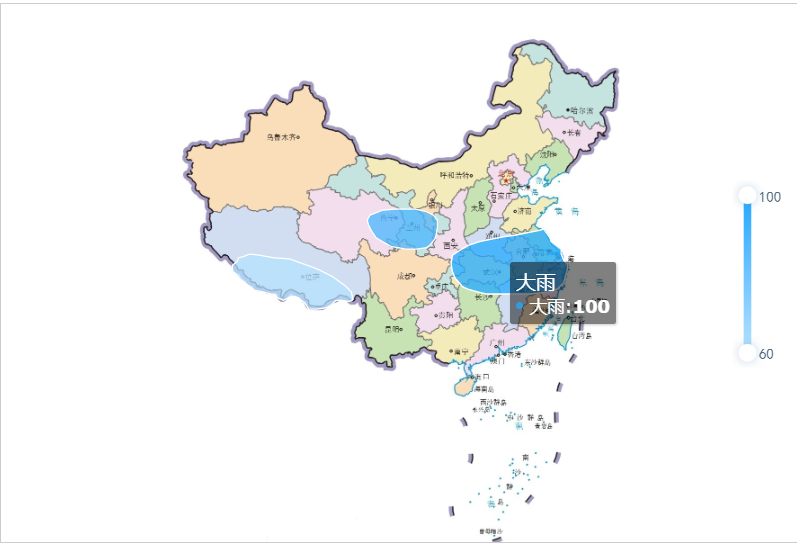
\includegraphics[width=0.60\textwidth]{figs/降雨.png}
	\caption{降雨专题图}
	\label{fig:jiangyu}
\end{figure}
\section{系统测试}
\subsection{功能测试}
功能测试是软件测试的一个分支,旨在验证软件应用程序的功能,而不管功能是否根据需求规范运行。通过给出适当的输入值,确定输出并使用预期输出验证实际输出来测试每个功能。本项目主要测试专题图对数据的展示功能是否符合要求。
1.河流专题图功能测试

河流专题图的功能测试主要是测试当鼠标指向河流的某一段时,会显示出河流的上中或下游,并且展示出河流的流量,并且流量大小会通过颜色深浅来表示,流量越大,颜色越深,对河流专题图所设置的测试数据如\ref{heliu}所示,当鼠标指向河流特定一段时会展示出与其相对应的数据,即表示测试成功。
\begin{table}[H]
	\centering
	\caption[河流数据]{河流预设数据展示表}
	\label{heliu}
	\begin{tabular}{cc}
		\toprule
		名称           & 流量(单位:立方米每秒)     \\
		\midrule
		黄河上游         & 1800 \\
		黄河中上游     & 1600   \\
		黄河中游      & 1500      \\
		黄河中下游      & 1400    \\
		黄河下游 & 1200      \\
		长江上游 & 33980      \\
		长江中游       & 30000    \\
		长江下游  & 28000      \\
		\bottomrule
	\end{tabular}
\end{table}
测试结果如图\ref{fig:ceshiheliu}所示,测试成功。
\begin{figure}[!htb]%关于这些编译器的配置和使用,请参阅相关说明资料。
	\centering
	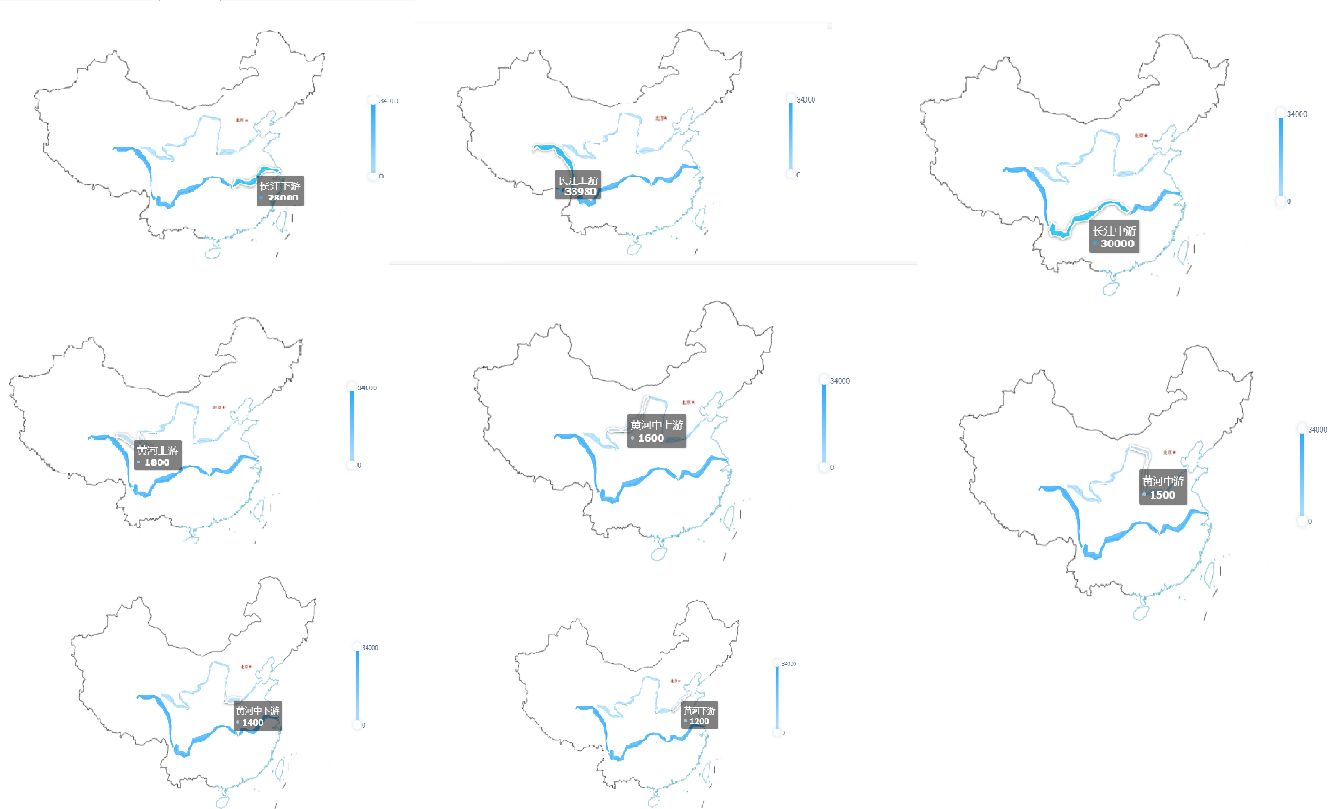
\includegraphics[width=0.60\textwidth]{figs/ceshiheliu.png}
	\caption{河流测试结果图}
	\label{fig:ceshiheliu}
\end{figure}

2.蓄水池专题图功能测试

蓄水池功能测试主要是打开蓄水池专题图时,会展示蓄水池的具体位置,以及蓄水量等信息。对蓄水池专题图所设置的测试数据如\ref{xushuici}所示,当展示位置和数据一致时,便为测试成功。
\begin{table}[H]
	\centering
	\caption[蓄水池数据]{蓄水池预设数据展示表}
	\label{xushuici}
	\begin{tabular}{cccc}
		\toprule
		名称           &经度 & 维度   & 含水量(单位:立方米)    \\
		\midrule
		1号蓄水池         & 116.143267&39.749144&100  \\
		2号蓄水池     & 108.034657  &32.081631 &49  \\
		3号蓄水池     & 108.074466 &34.28124&  94    \\
		4号蓄水池      & 113.535807 &34.81732&77    \\
		5号蓄水池   & 112.936703 &28.160166&88      \\
		6号蓄水池 & 118.045616 &24.366646&120      \\

		\bottomrule
	\end{tabular}
\end{table}

测试结果如\ref{fig:ceshixushuici}所示,测试成功。
\begin{figure}[!htb]%关于这些编译器的配置和使用,请参阅相关说明资料。
	\centering
	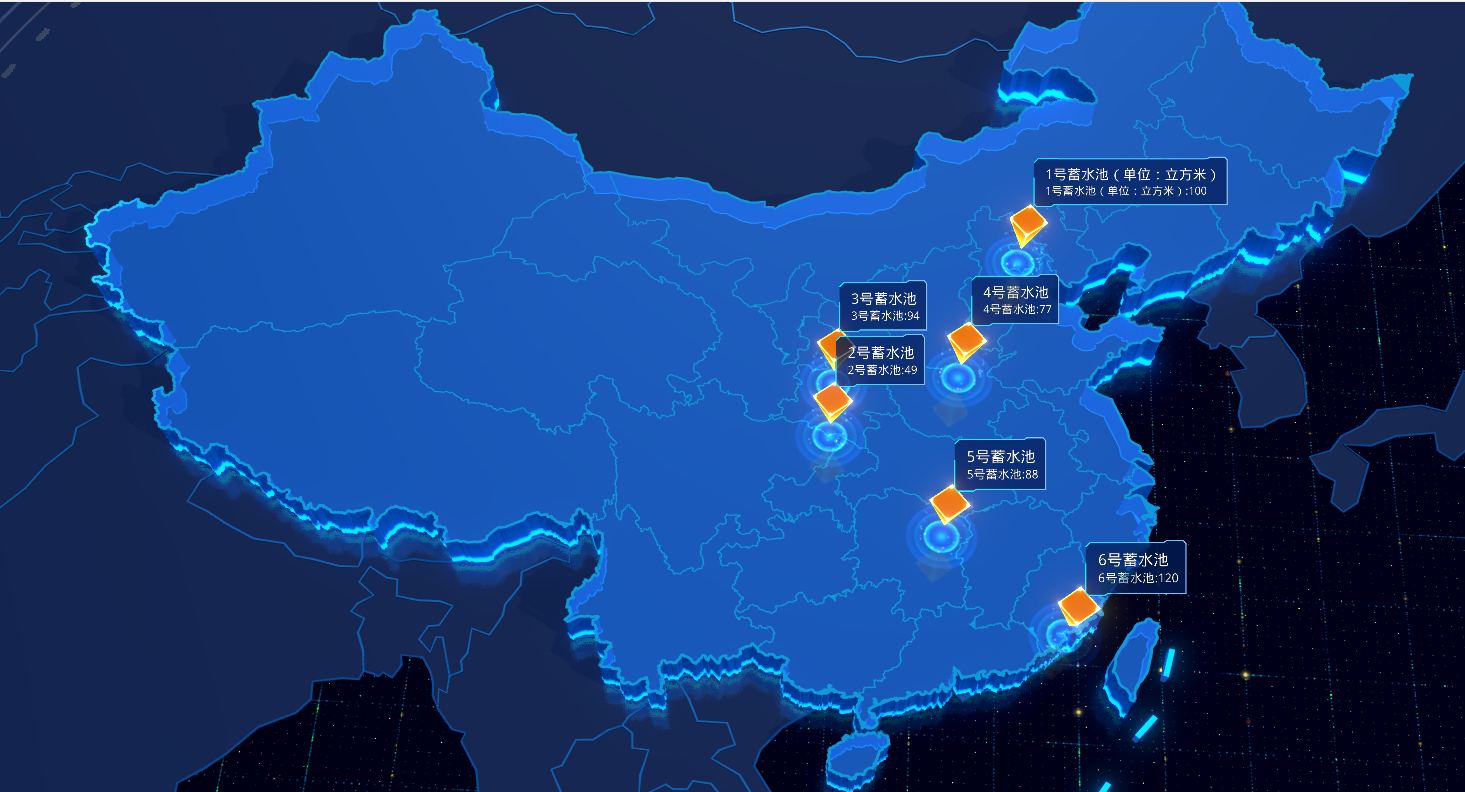
\includegraphics[width=0.60\textwidth]{figs/测试蓄水池.png}
	\caption{蓄水池测试结果图}
	\label{fig:ceshixushuici}
\end{figure}

3.地下水分布专题图功能测试。

地下水专题图功能测试主要是打开地下水专题图之后会展示各个省份所含有的地下水储量信息,对于地下水专题图所设置的测试数据如\ref{xushuici}所示,当数据能和专题图展示的信息相同,即测试成功。
\begin{table}[H]
	\centering
	\caption[地下水数据]{地下水预设数据展示表}
	\label{xushuici}
	\begin{tabular}{cc}
		\toprule
		省份          & 地下水含水量(单位:万立方米)    \\
		\midrule
		北京市        &425  \\
		山东省     &630 \\
		澳门特别行政区    &  541    \\
		台湾省     &587    \\
		
		
		\bottomrule
	\end{tabular}
\end{table}
测试结果如\ref{fig:ceshidixiashui}所示,测试成功。
\begin{figure}[!htb]%关于这些编译器的配置和使用,请参阅相关说明资料。
	\centering
	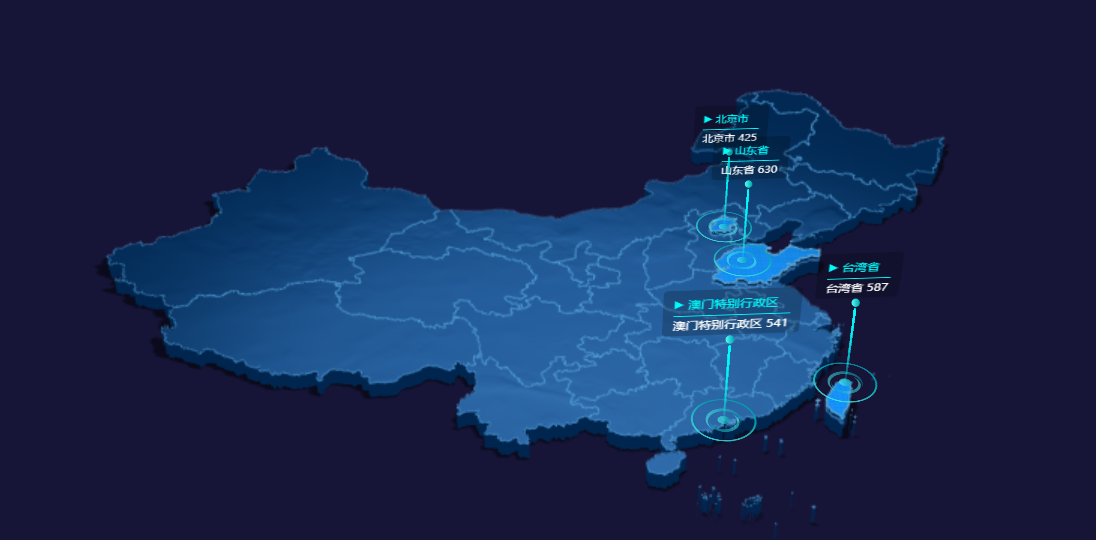
\includegraphics[width=0.60\textwidth,height=0.3\textheight]{figs/ceshidixiashui.png}
	\caption{地下水测试结果图}
	\label{fig:ceshidixiashui}
\end{figure}

4.对于降雨专题图,温度专题图,土壤类型和土壤含量专题图等的功能测试也是采用类似的方法,给专题图赋予数据之后,专题图根据各种预先设置的功能具体正确的展示给予的数据,便表示测试成功,经过对剩下的几种专题图的测试,发现结果和预想的结果全部相同,因此对于该项目的功能测试全部测试成功。
\subsection{非功能测试}
非功能测试是一种软件测试,用于测试非功能性参数,例如:软件的可靠性,负载测试,性能和责任等。非功能测试的主要目的是根据非功能参数测试软件系统的读取速度。

1.可靠性测试

对于软件使用者来说,期望软件能够没有错误的运行,对于本项目而言,可靠性主要为当数据改变时,专题图是否能够实时的展示出变化的数据,在测试过程中,当我们改变数据库的数据时,发现前端也跟随数据库的数据的变化而变化,并且变化的数据与修改的数据一致,因此得出结论,该项目比较可靠。

2.兼容性测试

本项目所进行的兼容性测试主要是测试在不同的浏览器上能否可以很好地运行,本项目主要使用了Firefox、Edge、Chrome、qq浏览器等,对于这些浏览器,本项目都可以在其上很好地运行。

3.负载测试

负载测试是要探讨在高峰或高于正常水平的负载下,系统或应用软件会发生什么情况。对于本项目而言,主要是测试最大支持多少并发用户数,对于本项目,我们使用了Apache的一个开源软件jMeter,用来测试负载能力,结果如\ref{fig:fuzaiceshi}所示,该项目的吞吐量为3376.857/minute,表示一分钟能处理3376.857次请求,结果较好,可以满足项目需求。

\begin{figure}[!htb]%关于这些编译器的配置和使用,请参阅相关说明资料。
	\centering
	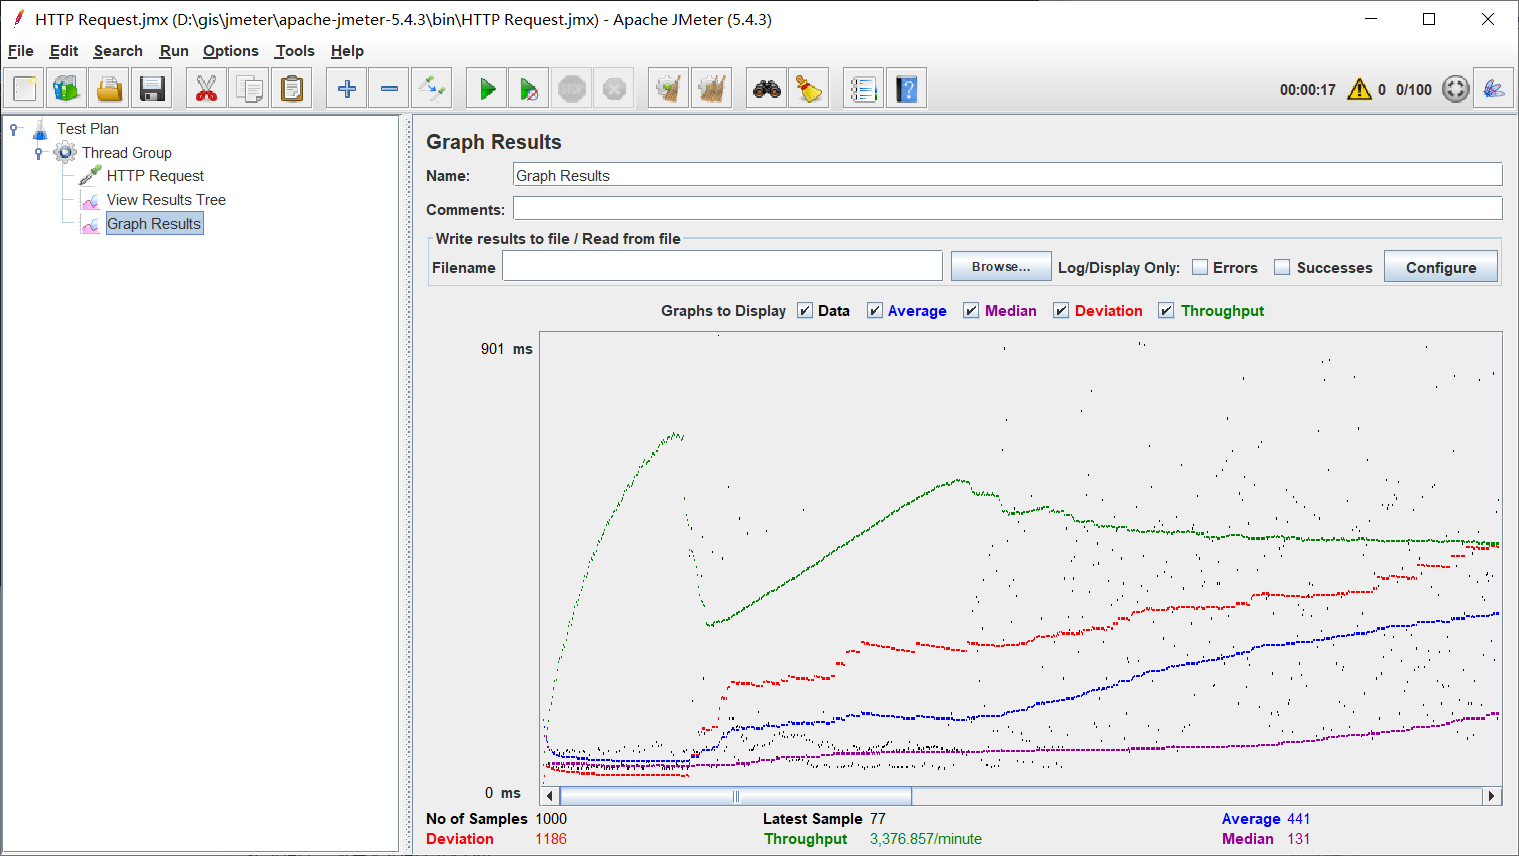
\includegraphics[width=0.60\textwidth,height=0.2\textheight]{figs/fuzaiceshi.png}
	\caption{负载测试结果图}
	\label{fig:fuzaiceshi}
\end{figure}
\begin{table}[H]
	\centering
	\caption[测试数据]{测试数据展示表}
	\label{test}
	\begin{tabular}{cc}
		\toprule
		操作          & 响应时间(单位:s)    \\
		\midrule
		打开专题图        &1.0  \\
		跳转到河流专题图     &0.03 \\
		跳转到蓄水池专题图    &0.21    \\
		跳转到水库专题图     &0.22    \\
		跳转到土壤专题图     &0.041    \\
		跳转到温度专题图     &0.021    \\
		跳转到降雨专题图     &0.033    \\
		
		
		\bottomrule
	\end{tabular}
\end{table}


4.压力测试

压力测试主要是为了测试硬件系统是否达到预期的性能目标,本项目主要测试了响应时间:打开专题图,跳转专题图等的响应时间。

主要响应时间如\ref{test}所示。由于蓄水池和水库专题图底图为3D底图,占用内存相对较大一些,因此响应时间相对来说较长一些,但是总体响应时间还是符合要求的。




%%% Local Variables: 
%%% mode: latex
%%% TeX-master: "../main.tex"
%%% End:
